\definecolor{classifierText}{HTML}{52575F}
\definecolor{bertBg}{HTML}{FFF5B5}
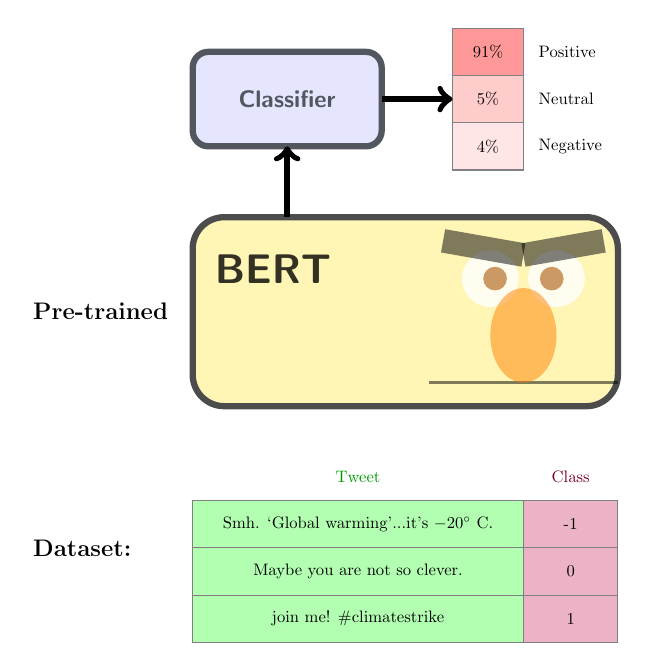
\begin{tikzpicture}[scale=0.6, every node/.style={scale=0.6}]
\node[font=\Large,anchor=west] at (-0.5,4) {\bfseries Dataset:};

% A
\filldraw[fill=green,draw=gray,fill opacity=0.3] (3,5) rectangle (10,4);
\node at (6.5,4.5) {Smh. `Global warming'...it's $-20^\circ$ C.};

\filldraw[fill=purple,draw=gray,fill opacity=0.3] (10,5) rectangle (12,4);
\node at (11,4.5) {-1};

% B
\filldraw[fill=green,draw=gray,fill opacity=0.3] (3,4) rectangle (10,3);
\node at (6.5,3.5) {Maybe you are not so clever.};

\filldraw[fill=purple,draw=gray,fill opacity=0.3] (10,4) rectangle (12,3);
\node at (11,3.5) {0};

\filldraw[fill=green,draw=gray,fill opacity=0.3] (3,3) rectangle (10,2);
\node at (6.5,2.5) {join me! \#climatestrike};

\filldraw[fill=purple,draw=gray,fill opacity=0.3] (10,3) rectangle (12,2);
\node at (11,2.5) {1};

\node[color=green!60!black] at (6.5,5.5) {Tweet};

\node[color=purple!60!black] at (11,5.5) {Class};

\node[font=\Large,anchor=west,text width=3cm] at (-0.5,9) {\textbf{Pre-trained}};

\filldraw[rounded corners=0.4cm,fill=bertBg,draw=black!70!white,line width=0.08cm] (3,11) rectangle (12,7);
\draw[thick, opacity=0.5] (8,7.5) -- (12,7.5);
\fill[color=white, opacity=0.8] (9.3,9.7) circle (0.6cm);
\fill[color=white, opacity=0.8] (10.7,9.7) circle (0.6cm);
\fill[color=brown, opacity=0.8] (9.4,9.7) circle (0.25cm);
\fill[color=brown, opacity=0.8] (10.6,9.7) circle (0.25cm);
\draw[line width=0.3cm, opacity=0.5] (8.3,10.5) -- (10,10.2);
\draw[line width=0.3cm, opacity=0.5] (10,10.2) -- (11.7,10.5);
\fill[color=orange, opacity=0.5] (10,8.5) ellipse (0.7cm and 1cm);
% \node at (10,8.5) {BERT};
\node[opacity=0.8] at (4.7,9.9) {\Huge \textsf{\textbf{BERT}}};

\filldraw[rounded corners=0.2cm,color=classifierText,fill=blue!10!white,line width=0.08cm] (3,14.5) rectangle (7,12.5);
\node[font=\Large] at (5,13.5) {\textcolor{classifierText}{\textsf{\textbf{Classifier}}}};

\draw[->,line width=0.08cm] (5,11) -- (5,12.5);

% Stuff
\filldraw[fill=red!40!white,draw=gray] (8.5,15) rectangle (10,14);
\node at (9.25,14.5) {91\%};

\filldraw[fill=red!20!white,draw=gray] (8.5,14) rectangle (10,13);
\node at (9.25,13.5) {5\%};

\filldraw[fill=red!10!white,draw=gray] (8.5,13) rectangle (10,12);
\node at (9.25,12.5) {4\%};

\node[anchor=west] at (10.2,14.5) {Positive};
\node[anchor=west] at (10.2,13.5) {Neutral};
\node[anchor=west] at (10.2,12.5) {Negative};

\draw[->,line width=0.08cm] (7,13.5) -- (8.5,13.5);
\end{tikzpicture}